Ce chapitre a pour but d'introduire quelques outils utiles pour l'analyse numérique (calcul d'intégrale et solution approchée d'une équation différentielle).

\section{Module \texttt{matplotlib.pyplot}}
	
	\subsection{Intérêt du module}

		Ce module permet d'afficher des dessins à l'écran au travers de diverses fonctions. On peut ainsi afficher des nuages de points de différentes couleurs ou formes, afficher des courbes ou des graphes etc.
	
		\python|matplotlib.pyplot| a la particularité de ne pas dessiner immédiatement à l'écran.
		C'est-à-dire que lorsqu'on demande l'affichage d'une figure (nuage de points, courbes etc) le programme n'affiche rien à l'écran~: les figures à dessiner sont stockées en mémoire et sont affichées sur demande (i.e. grâce à une autre fonction).
		
		Le nom du module étant particulièrement long, il est préférable de l'importer et de déclarer un alias~: \python|import matplotlib.pyplot as plt|
	
	\subsection{Fonctions usuelles}
		 
		 Deux fonctions sont indispensables~:
		 \begin{description}
		 	\item[\python|matplotlib.pyplot.show()|] affiche les figures stockées en mémoire
		 	\item[\python|matplotlib.pyplot.plot(X, Y)|] stocke en mémoire la courbe reliant les points de coordonnées $X_i~;\ Y_i$. (\python|X| et \python|Y| sont des listes ou des tableaux numpy)
		 \end{description}
		 
		 La fonction \python|matplotlib.pyplot.plot()| peut prendre bien d'autres arguments comme la couleur ou le style de points. Relativement peu utilisées, ces options ne sont pas à connaître.
		 
		 On peut également mentionner la fonction moins utilisée, mais néanmoins pratique~:\\\python|matplotlib.pyplot.scatter(X, Y)|. Elle permet de tracer un nuage de points sans les relier.
	
	\subsection{Exemples}
	
		Un petit script qui trace une courbe~:
		\begin{pythoncode}
			import matplotlib.pyplot as plt
			
			# Coordonnées des points
			X = [1, 2, 3, 4, 5]
			Y = [5, 2, 1, 3, 4]
			
			# Création de la courbe reliant les points
			plt.plot(X, Y)
			
			# Affichage de la courbe
			plt.show()
		\end{pythoncode}
		
		\begin{figure}[htp]
			\centering
			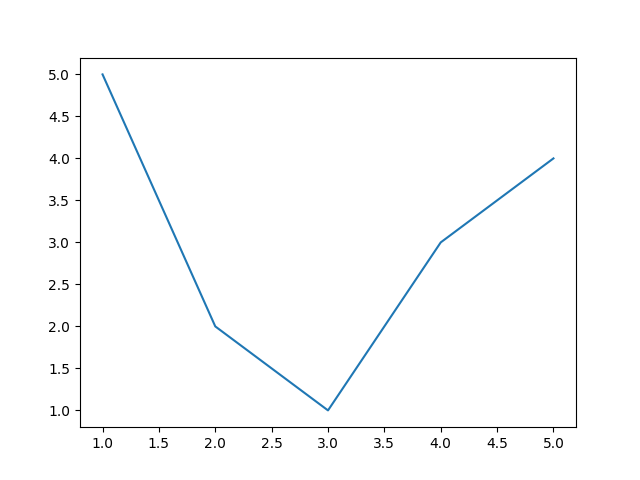
\includegraphics[scale=1.00]{images/Figure_1.png}
		\end{figure}
		
\section{Module \texttt{numpy}} \label{numpy}
	
	\subsection{Introduction au module}
		
		Le module \python|numpy| fourni non pas des fonctions, mais un nouveau type de variable~: le type \python|array|\footnote{Aussi parfois appelé "Tableau \python|numpy|"}.
		Ce type permet de construire des listes ou des tableaux de variables. Mais, contrairement aux listes Python, les \python|array| doivent respecter quelques règles~:
		\begin{itemize}
			\item la dimension est fixée lors de l'initialisation et ne peut pas être modifiée~;
			\item le type \python|array| ne peut contenir que des variables d'un seul type (e.g. on peut faire des \python|array| de \python|int|, de \python|str|, d'\python|array|, etc.).
		\end{itemize}
		En contrepartie de ces restrictions, le type \python|array| permet des manipulations plus agréables et intuitives.
		
		La dimension d'un tableau \python|numpy| est un tuple que l'on peut récupérer par la fonction~: \python|numpy.shape(mon_array)|\footnote{On pourrait également utiliser la syntaxe~: \python|mon_array.shape|.}. Si ce tuple ne contient qu'un seul nombre $n$, le tableau est unidimensionnel i.e. c'est une liste de longueur $n$~; s'il contient deux nombres $m$ et $n$, alors le tableau est bidimensionnel i.e. c'est une grille dotée de $m$ lignes et $n$ colonnes~; si la dimension est constituée de trois nombres, le tableau est dit tridimensionnel, et les trois nombres désignent sa largeur, sa hauteur et sa profondeur~; et ainsi de suite.
		
		On se contentera généralement de tableaux uni- ou bi-dimensionnels.
	
	\subsection{Tableaux \texttt{numpy}}
	
		\subsubsection{Initialisation}
		
		Il existe plusieurs méthodes d'initialisations.
		
		\subparagraph{En énumérant les éléments}
		Les tableaux \python|numpy| se comportent alors comme des listes Python, il faut donner les valeurs~: \python|numpy.array(data)|.
		Où \python|data| est une liste Python (ou un tuple). Pour un tableau bidimensionnel, \python|data| est une liste de listes de même longueur qui représentent chacune une ligne du tableau. Pour un tableau tridimensionnel, \python|data| est une liste de listes de listes, et ainsi de suite.
		
		\subparagraph{Avec la dimension}
		Si l'on connait la dimension exacte du tableau que l'on veut créer, on peut demander à \python|numpy| de construire un \python|array| de cette taille.
		Il faut alors préciser si l'on souhaite~:
		\begin{itemize}
			\item un tableau de 0~: \python|numpy.zeros(dimension)|, avec \python|dimension| la dimension du tableau souhaité, sous forme de tuple ou de liste.
			\item un tableau de nombre aléatoires~: \python|numpy.random.randint(minimum, maximum, dimension)|.
		\end{itemize}
		
		\subparagraph{Pour une courbe}
		Lorsque l'on veut calculer les points d'une courbe, on a souvent l'intervalle sur lequel il faut calculer les points et le pas\footnote{L'écart entre chaque points. Plus l'écart est grand, moins il y aura de points.}
		On utilise alors la fonction~:\\\python|numpy.arange(debut, fin, pas)|. À noter que comme pour le \python|range| du Python, la borne haute n'est pas atteinte.
		
		Dans certains cas, il est préférable de laisser \python|numpy| choisir le pas. Il faut alors lui donner un autre argument~: le nombre de points voulu.
		Il faut utiliser une autre fonction~: \python|numpy.linspace(debut, fin, nombre_points)|. Attention, ici la borne supérieure est atteinte.
	
		\subsubsection{Effets des opérateurs et fonctions}
		Les opérateurs sur les tableaux \python|numpy| ont une signification différentes de celle qu'ils ont sur les listes Python.
		
		En effet, sur les \python|array|, les opérateurs correspondent à des opérations terme à terme sur les éléments du tableau. Ainsi, additionner deux tableaux \python|numpy| revient à sommer terme à terme les éléments des tableaux. Pour avoir le droit d'effectuer une opération sur deux tableaux \python|numpy|, il faut donc que les deux tableaux soient de même dimension.
		On peut également additionner avec un scalaire pour ajouter la même valeur à toutes les cases. De même pour la soustraction, la multiplication, la division et la division euclidienne (quotient et reste).
		
		On peut également appliquer des fonctions mathématiques sur l'ensemble d'un tableau \python|numpy|.
		La syntaxe est alors plus complexe~: \python|numpy.vectorize(fonction)(tableau)|, où \python|fonction| est la fonction mathématique à appliquer sur \python|tableau|.
		
		\subsubsection{Extraction d'un sous-tableau}
		Comme pour les listes (voir~\ref{slicing}), on peut extraire un sous-tableau d'un tableau \python|numpy|, et on va là encore utiliser la syntaxe~: \python|tableau[debut: fin]|.
		La subtilité est qu'un tableau peut être $n$-dimensionnel. Il va donc falloir indiquer la zone à garder, et ce pour chaque dimension.
		
		La syntaxe est alors~: \python|tableau[debut_1: fin_1, debut_2: fin_2, ..., debut_n: fin_n]|.
		Comme pour les listes, l'indice de fin n'est jamais atteint et l'on peut utiliser des indices négatifs pour compter à partir de la fin.		
	
	\subsection{Exemples}
		
		\subsubsection{Initialisation}
		
		\begin{pythoncode}
			>>> import numpy as np
			>>> np.array([[1, 2], [3, 4]])
			array([[1, 2],
			       [3, 4]])
			>>> np.zeros((3))
			array([0., 0., 0.])
			>>> np.arange(0, 5, 0.5)
			array([0., 0.5, 1., 1.5, 2., 2.5, 3., 3.5, 4., 4.5])
		\end{pythoncode}
		
		\subsubsection{Manipulations élémentaires}
		
		\begin{pythoncode}
			>>> from math import cos
			>>> import numpy as np
			>>> tableau = np.array([[1, 2], [3, 4]])
			>>> tableau + 1
			array([[2, 3],
			       [4, 5]])
			>>> np.vectorize(cos)(tableau)
			array([[ 0.54030231, -0.41614684],
			       [-0.9899925 , -0.65364362]])
		\end{pythoncode}
		
		\subsubsection{Extraction d'un sous-tableau}
		
		\begin{pythoncode}
			>>> import numpy as np
			>>> tableau = np.array([[1, 2, 3], [4, 5, 6], [7, 8, 9]])
			>>> tableau
			array([[1, 2, 3],
			       [4, 5, 6],
			       [7, 8, 9]])
			>>> tableau[:, 0] # On ne garde que le premier élément de chaque ligne
			array([1, 4, 7])
			>>> tableau[1, 0]
			4
			>>> tableau[1:, 1:] # On garde tout à partir de la deuxième colonne et de la deuxième ligne
			array([[5, 6],
			       [8, 9]])
			>>> tableau[:2, 1:2] # On ne garde que les deux premières lignes de la deuxième colonne
			array([[2],
			       [5]])
			>>> tableau[:-1, 1:]
			array([[2, 3],
			       [5, 6]])
			>>> tableau[1:-1, 0]
			array([4])
		\end{pythoncode}
		
\section{Application}
	
	\subsection{Calcul des points d'une fonction et affichage} \label{appl:pts_fonction} (Corrigé~: \ref{corr:pts_fonction})
		
		À l'aide de deux tableaux \python|numpy|, calculez et tracez la fonction $f~:\ x \mapsto \frac{\sin(x)}{x}$. L'intervalle et le nombre de point sont laissés libre.
		Quelques grandes étapes~:
		\begin{enumerate}
			\item Choisir un intervalle sur lequel $f$ est définie et fixer un nombre de points.
			\item Commencer par créer un tableau pour les abscisses
			\item Construire le tableau pour les ordonnées
			\item Afficher le resultat
		\end{enumerate}
	
	